% This is the master file of the folder structure. In order to compile your document, run this file. In most LaTeX editors, the master file can be specified such that the document can also be compiled from the other .tex files (in the docs folder).

% First, the preamble needs to be called. This contains all the 'under the hood' stuff for your document.
% ******************************************************************************
% ****************************** Custom Margin *********************************

% Add `custommargin' in the document class options to use this section
% Set {innerside margin / outerside margin / topmargin / bottom margin}  and
% other page dimensions
\ifsetCustomMargin
  \RequirePackage[left=37mm,right=30mm,top=35mm,bottom=30mm]{geometry}
  \setFancyHdr % To apply fancy header after geometry package is loaded
\fi

% *****************************************************************************
% ******************* Fonts (like different typewriter fonts etc.)*************

% Add `customfont' in the document class option to use this section

\ifsetCustomFont
  % Set your custom font here and use `customfont' in options. Leave empty to
  % load computer modern font (default LaTeX font).
  %\RequirePackage{helvet}

  % For use with XeLaTeX
  %  \setmainfont[
  %    Path              = ./libertine/opentype/,
  %    Extension         = .otf,
  %    UprightFont = LinLibertine_R,
  %    BoldFont = LinLibertine_RZ, % Linux Libertine O Regular Semibold
  %    ItalicFont = LinLibertine_RI,
  %    BoldItalicFont = LinLibertine_RZI, % Linux Libertine O Regular Semibold Italic
  %  ]
  %  {libertine}
  %  % load font from system font
  %  \newfontfamily\libertinesystemfont{Linux Libertine O}
\fi

% *****************************************************************************
% **************************** Custom Packages ********************************

% ************************* Algorithms and Pseudocode **************************

%\usepackage{algpseudocode}


% ********************Captions and Hyperreferencing / URL **********************

% Captions: This makes captions of figures use a boldfaced small font.
%\RequirePackage[small,bf]{caption}

\RequirePackage[labelsep=space,tableposition=top]{caption}
\renewcommand{\figurename}{Fig.} %to support older versions of captions.sty


% *************************** Graphics and figures *****************************

%\usepackage{rotating}
%\usepackage{wrapfig}

% Uncomment the following two lines to force Latex to place the figure.
% Use [H] when including graphics. Note 'H' instead of 'h'
%\usepackage{float}
%\restylefloat{figure}

% Subcaption package is also available in the sty folder you can use that by
% uncommenting the following line
% This is for people stuck with older versions of texlive
%\usepackage{sty/caption/subcaption}
\usepackage{subcaption}

% ********************************** Tables ************************************
\usepackage{booktabs} % For professional looking tables
\usepackage{multirow}

%\usepackage{multicol}
%\usepackage{longtable}
%\usepackage{tabularx}


% *********************************** SI Units *********************************
\usepackage{siunitx} % use this package module for SI units


% ******************************* Line Spacing *********************************

% Choose linespacing as appropriate. Default is one-half line spacing as per the
% University guidelines

% \doublespacing
% \onehalfspacing
% \singlespacing


% ************************ Formatting / Footnote *******************************

% Don't break enumeration (etc.) across pages in an ugly manner (default 10000)
%\clubpenalty=500
%\widowpenalty=500

%\usepackage[perpage]{footmisc} %Range of footnote options


% *****************************************************************************
% *************************** Bibliography  and References ********************

%\usepackage{cleveref} %Referencing without need to explicitly state fig /table

% Add `custombib' in the document class option to use this section
\ifuseCustomBib
   \RequirePackage[square, sort, numbers, authoryear]{natbib} % CustomBib

% If you would like to use biblatex for your reference management, as opposed to the default `natbibpackage` pass the option `custombib` in the document class. Comment out the previous line to make sure you don't load the natbib package. Uncomment the following lines and specify the location of references.bib file

%\RequirePackage[backend=biber, style=numeric-comp, citestyle=numeric, sorting=nty, natbib=true]{biblatex}
%\bibliography{References/references} %Location of references.bib only for biblatex

\fi

% changes the default name `Bibliography` -> `References'
\renewcommand{\bibname}{References}


% ******************************** Roman Pages *********************************
% The romanpages environment set the page numbering to lowercase roman one
% for the contents and figures lists. It also resets
% page-numbering for the remainder of the dissertation (arabic, starting at 1).

\newenvironment{romanpages}{
  \setcounter{page}{1}
  \renewcommand{\thepage}{\roman{page}}}
{\newpage\renewcommand{\thepage}{\arabic{page}}}


% ******************************************************************************
% ************************* User Defined Commands ******************************
% ******************************************************************************

% *********** To change the name of Table of Contents / LOF and LOT ************

%\renewcommand{\contentsname}{My Table of Contents}
%\renewcommand{\listfigurename}{My List of Figures}
%\renewcommand{\listtablename}{My List of Tables}


% ********************** TOC depth and numbering depth *************************

\setcounter{secnumdepth}{2}
\setcounter{tocdepth}{2}


% ******************************* Nomenclature *********************************

% To change the name of the Nomenclature section, uncomment the following line

%\renewcommand{\nomname}{Symbols}


% ********************************* Appendix ***********************************

% The default value of both \appendixtocname and \appendixpagename is `Appendices'. These names can all be changed via:

%\renewcommand{\appendixtocname}{List of appendices}
%\renewcommand{\appendixname}{Appndx}

% *********************** Configure Draft Mode **********************************

% Uncomment to disable figures in `draftmode'
%\setkeys{Gin}{draft=true}  % set draft to false to enable figures in `draft'

% These options are active only during the draft mode
% Default text is "Draft"
%\SetDraftText{DRAFT}

% Default Watermark location is top. Location (top/bottom)
%\SetDraftWMPosition{bottom}

% Draft Version - default is v1.0
%\SetDraftVersion{v1.1}

% Draft Text grayscale value (should be between 0-black and 1-white)
% Default value is 0.75
%\SetDraftGrayScale{0.8}


% ******************************** Todo Notes **********************************
%% Uncomment the following lines to have todonotes.

%\ifsetDraft
%	\usepackage[colorinlistoftodos]{todonotes}
%	\newcommand{\mynote}[1]{\todo[author=kks32,size=\small,inline,color=green!40]{#1}}
%\else
%	\newcommand{\mynote}[1]{}
%	\newcommand{\listoftodos}{}
%\fi

% Example todo: \mynote{Hey! I have a note}


% The title page is created with the command \maketitle which needs to be placed after the \begin{document} command. To create the titlepage, some entries are needed: the name of the autor is defined by \author{}, the title by the entry \title{} and the date by the command \date{}. Note that the current date is displayed with \today.
\author{First von Last}
\title{Title of document}
\date{\today}

% All the actual content of your document should be placed after \begin{document} and before \end{document}. This content should be placed in the docs folder and can then be called with \input{docs/filename}.
\begin{document}

% Here the actual title page is printed, based on the given entries \author{}, \title{} and \date{}.
\maketitle

% The table of contents can be automatically generated with the \tableofcontents command. Note that you need to compile the document twice in order to see the changes in the table of contents.
\tableofcontents

% The \input{} command reads and processes the indicated example.tex file. Note that docs/ locates the folder where the .tex file is stored.
% A chapter named 'Your first document' is created
\chapter{Your first document} \label{cha:your-first-document}


% A section called 'Basics' is created
\section{Basics} \label{sec:basics}

Text is formatted with: \textbf{bold}, \textit{italic} and \underline{underline}.
\Cref{sec:basics} is part of \cref{cha:your-first-document}.


% A subsection named 'Typesetting content' is created
\section{Typesetting content} \label{sec:typesetting}


% A subsubsection named 'Equations' is created
\subsection{Equations} \label{subsec:equations}

% Inline equations
An example of an inline equation is: the derivative of $x^2$ is $2x$. \Cref{eq:example} shows a display equation:
% Display equations
\begin{align} \label{eq:example}
          y_{0} &= \frac{\sqrt{256}}{2} \\
                &= 2^{3} = 8 \nonumber 
\end{align}


\subsection{Units} \label{subsec:units}

% % Working with units
An easy way to work with (SI) units: \SI{1}{\hertz} is equal to \SI{2\pi}{\radian\per\second}.


\subsection{Figures} \label{subsec:figures}

% Inserting a figure
Here a figure named \textit{logo.pdf} is inserted\footnote{The \textit{logo.pdf} file is located in the figs folder.}:
\begin{figure}[h]
  \centering
  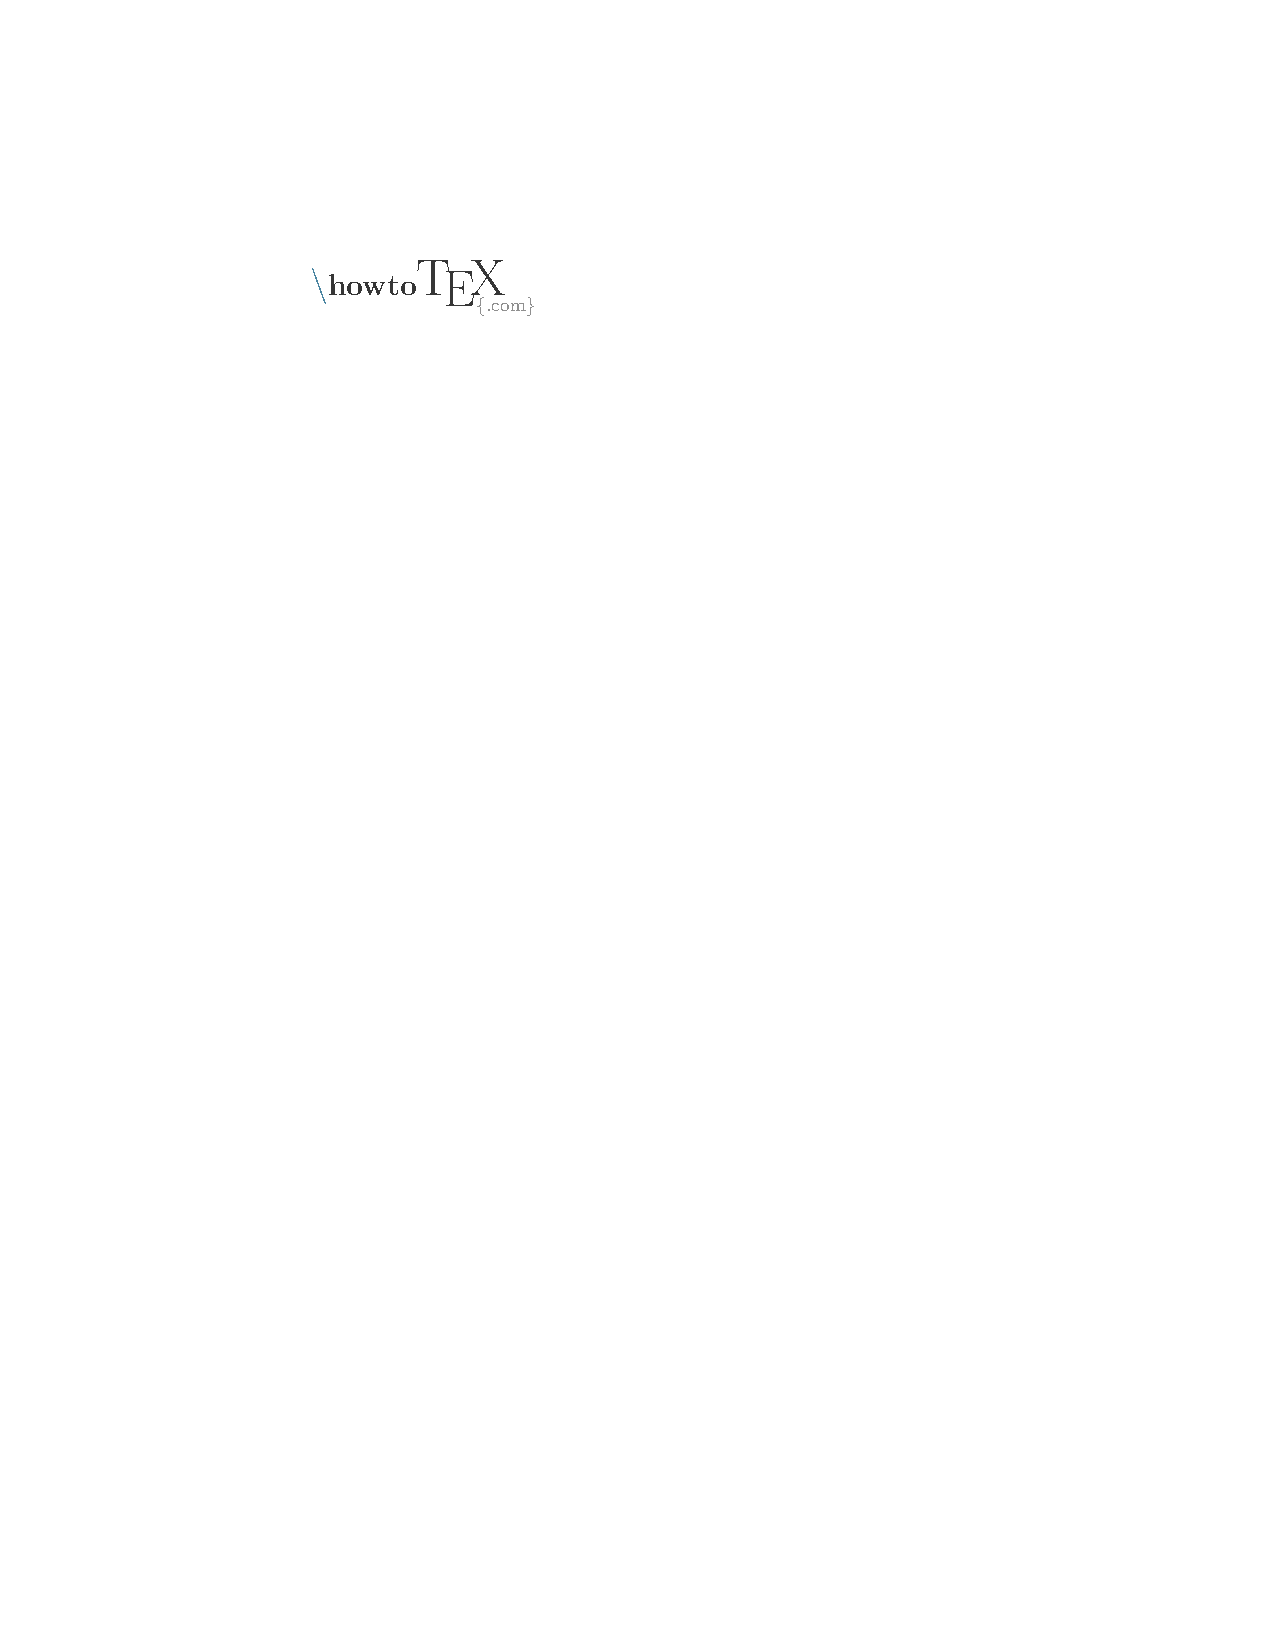
\includegraphics[width=50mm]{figs/logo}
  \caption{Caption example}
  \label{fig:logo}
\end{figure}


\subsection{Tables} \label{subsec:tables}

% Inserting a table
A table is shown in \cref{tb:table}.
\begin{table}[h]
  \centering
  \caption{Caption example}
  \label{tb:table}
  \begin{tabular}{crl}
    \toprule
    Name     & Grade & Year    \\
    \midrule
    John     & 7.5   & 2012\\
    Richard  & 2     & 2010\\
    \bottomrule
  \end{tabular}
\end{table}


\subsection{Lists} \label{subsec:lists}
% Creating lists
%% Here a subsubsection is created. Note that this section is not shown in the table of content.
\subsubsection{Numbered}
Creating a numbered list:
\begin{enumerate}
  \item First entry
  \item Second entry
\end{enumerate}

\subsubsection{Descriptive}
Creating a descriptive list:
\begin{description}
  \item[First] entry
  \item[Second] entry
\end{description}


\section{Reference to bibliography items} \label{sec:bibliography}
First are reference to a website is made \cite{MiscEntry}, then a reference to an article \cite{ArticleEntry} and finally a reference to a book \cite{last2012}.

\paragraph{Good luck!}

% The bibliography is printed with \bibliography{}. With the command \bibliographystyle{} a style is picked.
\bibliographystyle{plain}
\bibliography{refs/references}

% To close your document, add the \end{document} command. Everything after this command will not be processed.
\end{document}